\chapter{The superconducting qubit as an encoding surface}\label{ch:scprimer}

\section{The transmon}

A transmon is a Josephson junction, a thin AlO$_x$ tunnel barrier between two Al (or Nb, Ta)
electrodes, shunted by a large capacitance~\cite{Koch2007}. Its Hamiltonian
$H=4E_C(\hat n-n_g)^2-E_J\cos\hat\varphi$ at $E_J/E_C\sim50$ gives an anharmonic oscillator
with $\omega_q/2\pi\approx4$--$6$~GHz that is exponentially insensitive to charge noise. The
qubit state is carried by the phase of the superconducting condensate across the barrier.
In IAM terms the barrier is the encoding surface: it is where the condensate's phase can be
disturbed and where the information that constitutes the qubit state can be lost. The
transmon is now the working element of the largest processors~\cite{Arute2019,GoogleWillow2025,Kim2023IBM}.

\paragraph{Why the qubit is cold.} A superconducting processor is cooled to keep the qubit in its ground state and the metal superconducting.
At 5\,GHz and 15\,mK, $hf/k_BT=16.0$ and the thermal excited population $e^{-hf/k_BT}$ is $1.1\times10^{-7}$; at 50\,mK it is $8.2\times10^{-3}$
\calc. Aluminium is superconducting below $T_c\approx1.2$\,K: $\Delta_{\rm Al}=182\,\mu$eV gives $\Delta_{\rm Al}/(1.764\,k_B)=1.20$\,K \calc~\cite{Blais2021}.
The Landauer cost per bit is lower at 15\,mK as well, $1.44\times10^{-25}$\,J, by the ratio $0.015/300=5\times10^{-5}$ \calc, but lowering it is
not the purpose of the cooling; the cooling buys coherence. \interp

\paragraph{The qubit is hotter than its refrigerator.} The temperature that writes on a transmon is its own, not the mixing chamber's. In a
3D transmon whose refrigerator was swept from 150~mK down, the excited-state occupation followed a Maxwell--Boltzmann distribution at the
refrigerator temperature down to 35~mK and then saturated at 0.1\,\%, an effective qubit temperature of 35~mK~\cite{Jin2015} \observed. At
5~GHz that temperature gives $M=hf/\kB T=6.86$ and an equilibrium occupation of $1.1\times10^{-3}$, against $1.1\times10^{-7}$ at 15~mK
\calc. The floor this sets for a held record and for one gate is derived in Chapter~\ref{ch:qplatforms}.

\section{Three loss channels}

\paragraph{Two-level systems (TLS).} Amorphous oxides host atomic-scale tunnelling defects
with a broad distribution of energies and dipole moments~\cite{Phillips1987,Muller2019}. TLS
resonant with the qubit absorb energy. Off-resonant TLS that fluctuate, driven by their
thermal neighbours, produce spectral diffusion and dephasing. TLS density is highest at the
metal--oxide and substrate--air interfaces~\cite{Wang2015TLS,Lisenfeld2019}, and TLS switching
times span microseconds to hours.

\paragraph{Quasiparticles.} At $T\ll T_c$ the equilibrium density of broken Cooper pairs is~\cite{Glazman2021}
\begin{equation}
 \xqp^{\mathrm{th}}(T)=\sqrt{\frac{2\pi\kB T}{\Delta}}\,e^{-\Delta/\kB T}
\end{equation}
in the normalization $\xqp=n_{\mathrm{qp}}/\ncp$ with $\ncp=2\nu_0\Delta$ (Chapter~\ref{ch:xqp}).
At 15~mK in Al, $\Delta/\kB T=141$ and $\xqp^{\mathrm{th}}\sim10^{-62}$ \calc: there should be no
quasiparticles at all. Measured densities in transmons are commonly
$\xqp\sim10^{-8}$--$10^{-6}$~\cite{Riste2013,Serniak2018}, the best reported devices reach
$\xqp\lesssim10^{-9}$~\cite{Connolly2024}, and less-protected devices reach
$10^{-6}$--$10^{-5}$~\cite{Martinis2009,deVisser2011} \observed. The source of this non-equilibrium
population is the subject of Chapter~\ref{ch:xqp}. A quasiparticle tunnelling across the
junction relaxes the qubit at the rate~\cite{Catelani2011}
\begin{equation}
 \Gamma_1^{\mathrm{qp}}=\xqp\,\frac{\omega_q}{\pi}\sqrt{\frac{2\Delta}{\hbar\omega_q}} .
 \label{eq:catelani}
\end{equation}

\paragraph{Radiation and environment.} Ionizing radiation from the environment and from cosmic
rays deposits energy in the substrate. The resulting phonons break pairs and cause correlated
error bursts~\cite{Vepsalainen2020,Cardani2021,McEwen2022}. Infrared photons leaking into the
cryostat break pairs directly~\cite{Barends2011,Houzet2019}. Shielding, phonon traps,
gap engineering and underground operation mitigate these channels~\cite{Cardani2021,Martinis2021,Kurter2022}.
\paragraph{Which radiation reaches the junction.} A photon breaks a Cooper pair in aluminium only if $h\nu>2\Delta$,
that is $\nu>88$~GHz for $\Delta=182~\mu$eV \calc. Figure~\ref{fig:pairbreaking} gives the number of such photons
radiated by a black surface at temperature $T$. At the 15~mK of the mixing chamber the flux is
$5\times10^{-109}$~s$^{-1}$\,m$^{-2}$, zero for every purpose. At 4~K it is $8\times10^{16}$, at 50~K $2\times10^{20}$
and at 300~K $4\times10^{22}$~s$^{-1}$\,m$^{-2}$ \calc. The cosmic microwave background at 2.725~K would supply
$2\times10^{16}$~s$^{-1}$\,m$^{-2}$ above the aluminium threshold, but it never reaches the chip: the cryostat's 4~K,
50~K and room-temperature shields lie between, are each brighter above 88~GHz, and are what the filtering and shielding
have to stop. The pair-breaking sources that matter in practice are stray radiation from warmer stages leaking through
wiring and seams~\cite{Barends2011,Liu2024PBP}, and ionizing radiation, mainly cosmic-ray muons at about
1~cm$^{-2}$\,min$^{-1}$ at sea level~\cite{PDG2022} and gamma rays from the laboratory, which deposit energy in the
substrate~\cite{Vepsalainen2020,Cardani2021,McEwen2022}. A deposit of 100~keV can break at most
$10^{5}~\mathrm{eV}/2\Delta\approx2.7\times10^{8}$ pairs; phonons lose much of the energy before it reaches the films,
so this is an upper bound \calc. Tantalum ($2\Delta/h\approx330$~GHz) and niobium ($\approx680$~GHz) need hotter
radiators for the same flux.
\paragraph{Where each surface sits against the background.} Every physical system sits somewhere relative to the cosmic
microwave background at $T_{\rm CMB}=2.7255$~K (Figure~\ref{fig:temp_ladder}). A transistor junction at 75\,$^\circ$C is 128 times
hotter, a cell at 37\,$^\circ$C is 114 times hotter, and a superconducting qubit at 15~mK is 182 times colder \calc. A solar-mass
black hole, at $T_H=61.7$~nK, is $4.4\times10^{7}$ times colder: the background writes on it rather than the other way round, and it
grows by absorbing the background unless its mass is below $4.5\times10^{22}$~kg (Chapter~\ref{ch:saturation}) \calc. Heat flows from
the hotter side to the colder one, so a surface colder than its surroundings is the one being written on \interp. For the qubit the
surroundings are not the sky but the cryostat. The background carries $3.13\times10^{-6}$~W\,m$^{-2}$ in all, of which
$2.81\times10^{-6}$~W\,m$^{-2}$ (89.8\,\%) lies above the aluminium threshold, in $2.18\times10^{16}$ photons s$^{-1}$\,m$^{-2}$ of mean
energy $\kB\times9.31$~K, enough for at most 2.2 broken pairs per photon \calc. None of it reaches a shielded chip. What writes on a cold
qubit is, in order: the defects of the substrate and its oxides, the TLS that limit $T_1$
(Chapter~\ref{ch:walls}); residual thermal photons from warmer stages leaking through wiring and seams; and cosmic-ray muons and gamma
rays, which no cryostat stops \observed. The first is a property of the material, the second an engineering limit, and the third is
reduced only underground.

\begin{figure}[htbp]\centering
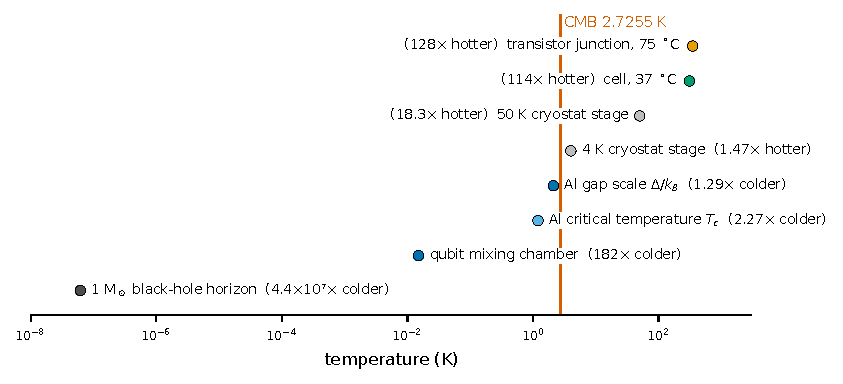
\includegraphics[width=\textwidth]{figures/part3/fig_p3_temperature_ladder.pdf}
\caption{The surfaces of Part~\ref{part:3} and their neighbours on one temperature axis, each against the cosmic microwave background
(2.7255~K): a solar-mass horizon (61.7~nK), the qubit's mixing chamber (15~mK), the critical temperature and gap scale of aluminium
(1.20 and 2.11~K), the 4~K and 50~K stages of the cryostat, a cell at 37\,$^\circ$C and a transistor junction at 75\,$^\circ$C. \calc}
\label{fig:temp_ladder}
\end{figure}

\begin{figure}[htbp]\centering
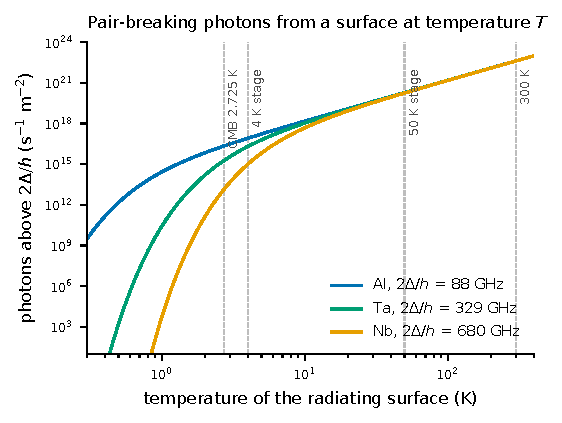
\includegraphics[width=0.62\textwidth]{figures/part3/fig_p3_pairbreaking.pdf}
\caption{Photons with $h\nu>2\Delta$ radiated into a hemisphere per second and per square metre by a black surface at
temperature $T$, for Al, Ta and Nb ($\Delta=1.764\,\kB T_c$ with $T_c=1.2$, 4.47 and 9.25~K). Dashed lines: the
cosmic microwave background, the 4~K and 50~K stages of a dilution cryostat, and room temperature. \calc\ (Planck
law, BCS gap)}\label{fig:pairbreaking}
\end{figure}

\section{The $T_1$ ceiling from quasiparticles}

\calc\ Equation~\eqref{eq:catelani} with $\Delta_{\mathrm{Al}}=182\ \mu$eV and $\omega_q/2\pi=5$~GHz
gives $T_1^{\mathrm{qp}}=0.24$~ms at $\xqp=10^{-7}$, and 1~ms requires $\xqp\le2.4\times10^{-8}$
(Figure~\ref{fig:T1xqp}). The simpler estimate $\Gamma_1^{\mathrm{qp}}\approx\xqp\,\omega_q$ gives 0.32~ms.
The best transmons now reach $T_1\sim0.3$--$0.5$~ms~\cite{Place2021,Wang2022Ta}; for Al at 5~GHz
that requires $\xqp\le8\times10^{-8}$ and $\le5\times10^{-8}$ respectively \calc. Whatever sets the
background $\xqp$ therefore sets a limit close to present superconducting-qubit coherence.
Table~\ref{tab:T1xqp} gives the ceiling across the measured range of $\xqp$ at two qubit frequencies.
% generated by docs/book/figscripts/fig_p3_extra.py; do not edit by hand
\begin{table}[htbp]\centering\small
\caption{Quasiparticle-limited $T_1$ of an Al transmon ($\Delta_{\rm Al}=182\,\mu$eV) from Eq.~\eqref{eq:catelani} at two qubit frequencies, and the simpler estimate $\Gamma_1^{\rm qp}\approx\xqp\,\omega_q$ at 5~GHz. The first two rows bracket the 1~ms target; the range $10^{-8}$--$10^{-6}$ is the measured background of best-isolated devices~\cite{Riste2013}. \calc}\label{tab:T1xqp}
\begin{tabular}{@{}lccc@{}}\toprule
$\xqp$ & $T_1^{\rm qp}$ (ms), 4~GHz & $T_1^{\rm qp}$ (ms), 5~GHz & $1/(\xqp\omega_q)$ (ms), 5~GHz \\\midrule
$1.0\times10^{-8}$ & 2.66 & 2.38 & 3.18 \\
$2.4\times10^{-8}$ & 1.11 & 0.993 & 1.33 \\
$1.0\times10^{-7}$ & 0.266 & 0.238 & 0.318 \\
$1.0\times10^{-6}$ & 0.0266 & 0.0238 & 0.0318 \\
$1.0\times10^{-5}$ & 0.00266 & 0.00238 & 0.00318 \\
\bottomrule
\end{tabular}
\end{table}

Coherence time is not by itself an error-correction requirement. The surface code needs the error per operation to
lie below a threshold of about $10^{-2}$~\cite{Fowler2012}, and the 105-qubit processor of Ref.~\cite{GoogleWillow2025}
operated below threshold with a mean $T_1$ of $68~\mu$s and a mean $T_{2,\mathrm{CPMG}}$ of $89~\mu$s \observed. A
longer $T_1$ lowers the error per operation and the code overhead; it is not a gate that must be passed first. The
ratio $T_2/T_1=1.31$ lies within the bound $T_2\le2T_1$ \calc.

\begin{figure}[htbp]\centering
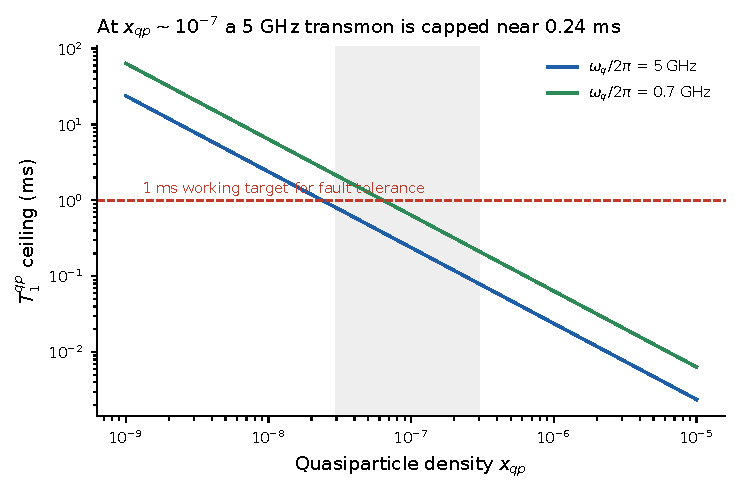
\includegraphics[width=0.75\textwidth]{figures/part3/fig_T1_xqp.pdf}
\caption{Quasiparticle-limited $T_1$ from Eq.~\eqref{eq:catelani} for Al at two qubit
frequencies. Grey band: the range of background $\xqp$ commonly reported in transmons. Dashed:
1~ms working target. \calc}\label{fig:T1xqp}
\end{figure}

\section{Timescales at a junction}
\begin{center}\begin{minipage}{\linewidth}\centering
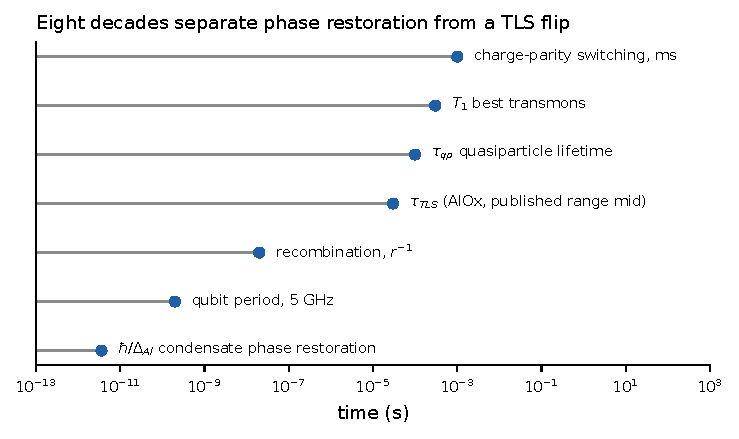
\includegraphics[width=0.52\textwidth]{figures/part3/fig_timescales.pdf}
\captionof{figure}{Timescales at an Al/AlO$_x$ junction, from condensate phase restoration to
charge-parity switching. \calc\ and \observed\ (representative published values).}
\label{fig:timescales}
\end{minipage}\end{center}

The IAM argument of Chapter~\ref{ch:xqp} rests on a separation of timescales
(Figure~\ref{fig:timescales}). The condensate restores its phase on $\hbar/\Delta_{\mathrm{Al}}$.
The qubit oscillates at $\sim0.2$~ns. Quasiparticles recombine on tens of ns to ms depending
on density, TLS fluctuate on $\mu$s and longer, and $T_1$ is hundreds of $\mu$s.

\begin{checkbox}
$\hbar/\Delta_{\mathrm{Al}}=1.055\times10^{-34}/(182\times10^{-6}\times1.602\times10^{-19})=3.6\times10^{-12}$~s,
that is \textbf{3.6~ps}. Against TLS switching times of 1--100~$\mu$s the ratio $\tau_\phi/\tTLS$ is
$4\times10^{-6}$ to $4\times10^{-8}$. The separation spans five to seven decades, so each TLS flip is a
Markovian event for the condensate. \calc
\end{checkbox}

A device physicist can measure $\xqp$ on their own junction, put it into Eq.~\eqref{eq:catelani}, and compare with the measured $T_1$. That comparison is where the next gain in coherence is found.
